%%
%% Author: dariochinelli
%% 2021-04-08
%%


\section{Condensazione di Bose-Einstein}
Considero un gas di bosoni, la statistica che lo regola è 
\begin{equation}
\frac{n_s}{g_s} = \frac{1}{e^{ \alpha + \beta E_s } - 1}
\end{equation}
ed imponendo che i parametri di Lagrange siano
\begin{equation}
\beta = \frac{1}{k_B T} \quad\quad\quad \alpha > 0
\end{equation}
trovo che a temperatura $T = \SI{0}{K}$ solo gli stati con $E_s = 0$ sono occupati, assumendo $g_0  = 1$ trovo
\begin{equation}
N \simeq \frac{ 1}{e^{ \alpha } - 1 }
\label{N_alpha}
\end{equation}
ed invertendo trovo la relazione
\begin{equation}
e^{\alpha} = 1 + \frac{1}{N} \simeq 1 \quad \mbox{quando } N \to \infty
\end{equation}
per cui il sistema è degenere.
Essendo $\alpha \to 0$ posso sviluppare la \ref{N_alpha} come
\begin{equation}
N \simeq \frac{1}{1+ \alpha - 1} = \frac{1}{\alpha}
\end{equation}
lasciando esplicito $g_0$ avrei
\begin{equation}
n_0 \simeq N \simeq \frac{g_0}{e^{ \alpha } - 1 }
\quad\quad
e^{\alpha} = 1 + \frac{g_0}{N} \simeq 1
\quad\quad
N \simeq \frac{g_0}{\alpha}
\end{equation}

La relazione 
\begin{equation}
e^{\alpha} \simeq 1
\end{equation}
resta valida anche a $T \not= 0$ vicina allo zero assoluto, per cui posso chiedermi quante particelle sono all'energia \emph{ground state} $E_s = 0$?
Cerco un'espressione per $n_0$, il ground state, in funzione della temperatura
\begin{equation}
N = \sum_s n_s = n_0 (T) + n_e(T)
\end{equation}
ovvero la somma tra il numero di particelle nello stato fondamentale più il numero di particelle in tutti gli altri stati, stati eccitati.
Utilizzo l'equazione al continuo per la legge di Bose Einstein e la funzione densità degli stati 
\begin{equation}
\begin{split}
n(E)dE & = g(E) \frac{ 1}{e^{ \alpha + E / k_B T } - 1 } dE \\
g(E)dE & = \frac{4\pi V (2m^3)^{ \frac{1}{2} }}{h^3} E^{ \frac{1}{2} } dE
\end{split}
\end{equation}
e quindi integro nell'intervallo $\Bigl[  0, \infty  \Bigr]$
\begin{equation}
\begin{split}
N & = n_0 + \int_0^{\infty} n(E)dE \\
& = n_0 + c \int_0^{\infty} \frac{E^{ \frac{1}{2} }}{e^{ \alpha + \beta E } - 1} dE
\end{split}
\end{equation}
in cui ho sostituito e sostituisco
\begin{equation}
\begin{split}
& c = \frac{4\pi V (2m^3)^{ \frac{1}{2} }}{h^3} \\
& z= \beta E \quad\quad\quad dE = \frac{dz}{\beta} = dz k_B T
\end{split}
\end{equation}
e ottengo
\begin{equation}
N = n_0 + c(k_B T)^{\frac{3}{2}} G(\alpha)
\label{N_di_gamma}
\end{equation}
definendo la funzione \emph{gamma}
\begin{equation}
G(\alpha) = \int_0^{\infty} x^{ \frac{1}{2} } (e^{ z + \alpha } - 1) dz
\end{equation}
Se $\alpha$ è grande
\begin{equation}
\begin{split}
G(\alpha) & = e^{ - \alpha} \int_0^{\infty} x^{ \frac{1}{2} } e^{ -z } dz \\
G(\alpha) & \to e^{-\alpha} \frac{\sqrt{\pi}}{2}
\end{split}
\end{equation}
Se $\alpha$ è piccolo
\begin{equation}
\begin{split}
& G(0) \to 2.612 \frac{\sqrt{\pi}}{2} \\
& \alpha \simeq \frac{1}{N} \to 0 \quad\Rightarrow\quad G(\alpha) \approx G(0)
\end{split}
\end{equation}
allora l'equazione \ref{N_di_gamma} diventa
\begin{equation}
\begin{split}
N = n_0 + c (k_B T)^{ \frac{3}{2} } G(\alpha)
\quad\Rightarrow\quad 
n_0 & = N -  c (k_B T)^{ \frac{3}{2} } G(0) \\
& = N -  c (k_B T)^{ \frac{3}{2} } 2.612 \frac{\sqrt{\pi}}{2}
\end{split}
\end{equation}

Dalla formula 
\begin{equation}
\frac{n_0}{N} = 1 - \Bigl(  \frac{T}{T_C}  \Bigr)^{ \frac{3}{2} } 
\label{n0N}
\end{equation}
crivo la temperatura critica come
\begin{equation}
\begin{split}
T_C & = \frac{1}{k_B} \Bigl(  \frac{2N}{c \sqrt{\pi} 2.612}  \Bigr)^{ \frac{3}{2} } \\
&= \frac{2\pi \hbar^2}{k_B m} \Bigl(  \frac{N/V}{2.612}  \Bigr)^{ \frac{3}{2} } \propto \rho^{ \frac{3}{2} }
\end{split}
\end{equation}
quindi la temperatura critica è proporzionale alla densità elevata alla due terzi,
Plottando la relazione \ref{n0N} di $\frac{n_0}{N}$ si trova 
%% PLOT
Dalla temperatura critica $T_C$ diminuendo la temperatura tutte le particelle iniziano ad affollare lo stato fondamentale.
Che coincide alla \emph{condensazione di Bose Einstein}: tutte le particelle occupano lo stato fondamentale.








\newpage
Consideriamo bosoni con spin $= 0$ e massa $m \not = 0$ non interagenti.
Tutte le particelle tendono ad andare nel livello $E_s=0$.
\begin{equation}
\begin{split}
\frac{ n_s}{g_s } & = \frac{ 1}{e^{ \alpha + \beta E_s } - 1 } \\
\Rightarrow \frac{ n_0}{g_0 } & = \frac{ 1}{e^{ \alpha + \beta E_0 } - 1 } = \frac{ n_0}{g_0 } = \frac{ 1}{e^{ \alpha } - 1 } \\
\Rightarrow N & = \frac{ 1}{e^{ \alpha } - 1 }
\end{split}
\end{equation}

Notare che $g_0 = 1$ poiché $g(E) \sim E^{ \frac{ 1}{2 }}$ ma poiché $g(0)=0$ non ha senso fisico si assume che il minimo valore di $g$ sia 1.

Dato che $N$ (numero di particelle) è grande, allora, essendo $e^{ \alpha } = 1 + \frac{ 1}{N }\simeq 1 \Rightarrow \alpha \sim 0$ allora:
$$ N \simeq \frac{ 1}{1 + \alpha - 1 } \Rightarrow \alpha \simeq \frac{ 1}{N }$$
Il numero totale di particelle è dato da $N = \sum_s n_s = n_0 + n_e = n_0 + \int_0^{\infty} n(E)dE$ dove $n_0$ è il numero di particelle nello stato fondamentale e $n_e$ il numero di particelle negli stati eccitati.
Poiché però:
\begin{equation}
n(E)dE = \frac{ g(E)dE}{e^{ \alpha + \beta E_s } - 1 } \quad \mbox{ e } \quad g(E) dE= \frac{ 4 \pi V (2m^3)^\frac{ 1}{2 } E^\frac{ 1}{2 } }{ h^3} dE
\end{equation}

\begin{equation}
\begin{split}
N & = n_0 + C \int_0^{\infty} \frac{ E^{ \frac{ 1}{2 } }}{e^{\alpha + \beta E } -1 }dE = n_0 + C (kT)^{ \frac{ 3}{2 } } \int_0^{\infty} \frac{ z^{\frac{ 1}{2 } dz}}{e^{z+\alpha } - 1} \quad
\mbox{dove} \quad
\begin{cases}
	z = \beta E \\
	dE = k T dZ
\end{cases}
\end{split}
\end{equation}
Questo integrale, che chiameremo $G(\alpha)$, è estremamente complicato, ma si ha che:
\begin{equation}
\begin{cases}
	\alpha \mbox{ grande} \quad G(\alpha) = \frac{ \sqrt{\pi}}{2 } e^{ - \alpha } \\
	\alpha \mbox{ piccolo} \quad G(0) = 2.612 \sqrt{\frac{ \pi}{4 }}
\end{cases}
\end{equation}
Nel nostro caso $\alpha$ è piccolo essendo $N$ grande, e dunque si può approssimare scrivendo che 
\begin{equation}
\begin{split}
	n_0 & = N - C (kT)^{ \frac{ 3}{2 } } \sqrt{\frac{ \pi}{4 }} 2.612 = N \Bigl[ 1 - \frac{ T}{T_c } \Bigr] \\
	\mbox{dove } T_c & = (CN)^{ \frac{ 3}{2 } }  = C \Bigl(  \frac{ N}{V }  \Bigr)^{ \frac{ 3}{2 } } \sim e^{ \frac{ 3}{2 } } 
\end{split}
\end{equation}
per cui $T_c$ è una \underline{temperatura critica} che va come la densità alla $\frac{ 2}{3 }$.

	\newpage

\begin{figure}[h]
\centering
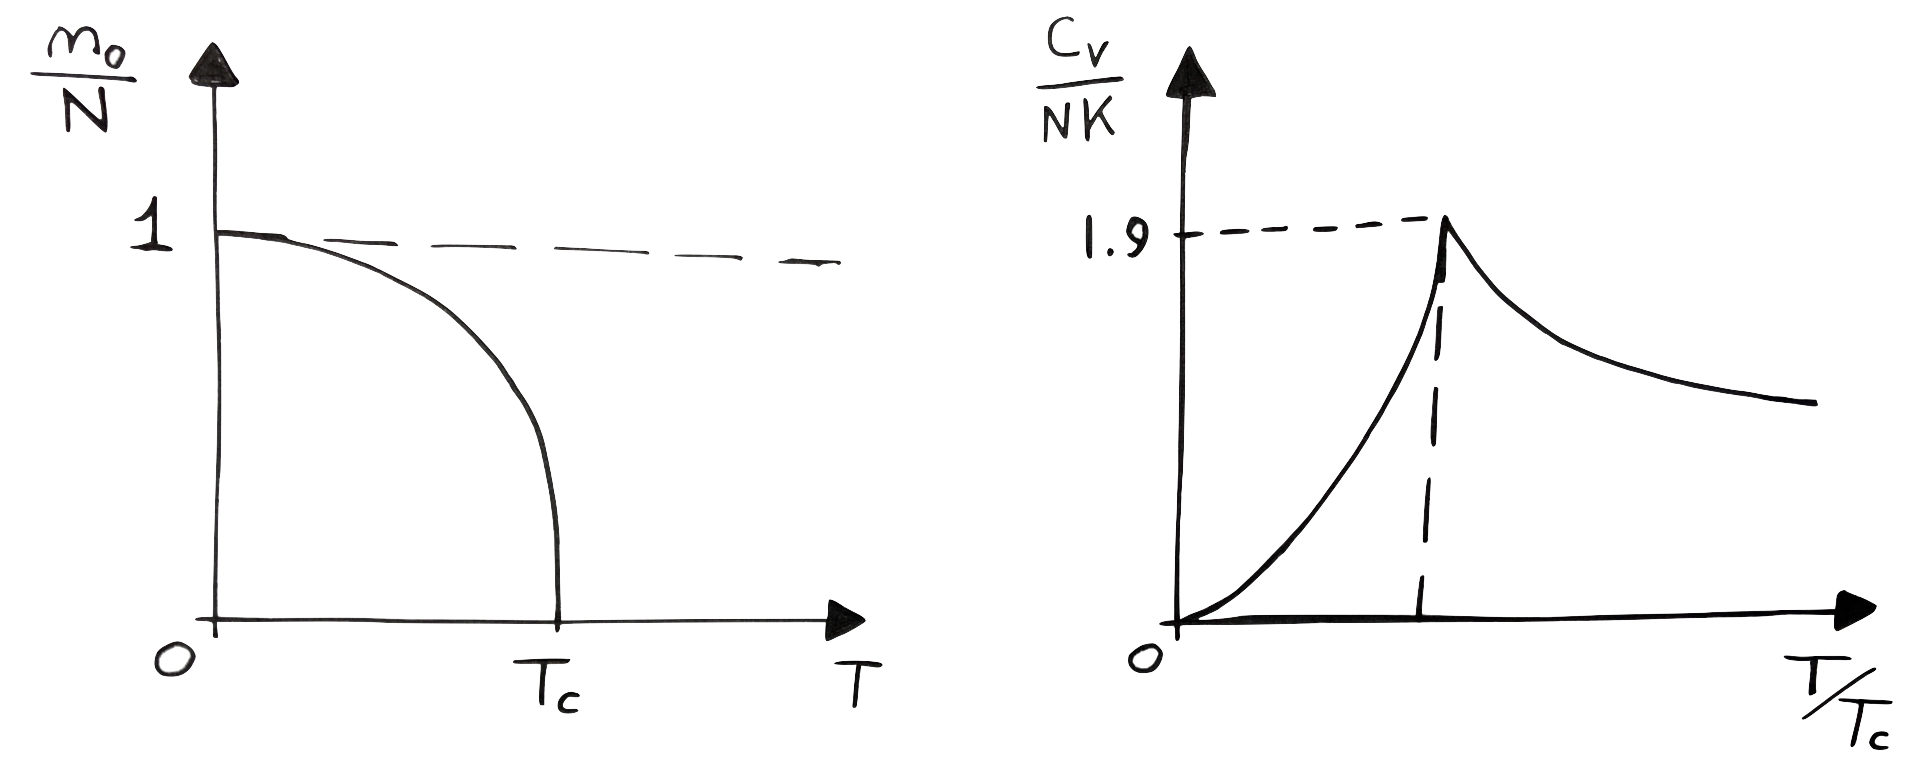
\includegraphics[scale=0.25]{/andamenti_Cv_T}
\end{figure}
Il numero di particelle nello stato fondamentale rimane grande fino a che $T < T_c$.
Al di sotto della temperatura critica le particelle sono condensate nel livello energetico minore di energia, cioè si ha il fenomeno della \underline{condensazione di Bose-Einstein}.
\begin{equation}
C_V = N K \Bigl(  \frac{ T}{T_c }  \Bigr) C \quad \mbox{dove} \quad C \to 1.9
\end{equation} 

Un fenomeno affascinante, affine alla condensazione di Bose-Einstein, è la superconduttività dell'elio liquido, per cui si consiglia di leggere il seguente paragrafo:

\textit{"Bose Condensation and liquid helium", pag 399-404, da Eisnerg-Resnick, Quantum Physics of atoms, molecules, solids, nuclei and particles}.


